\chapter{Heart Sound Modeling}


\section{Introduction}
The goal of this module is to create a model of the human heart. It should return 6 signals, one for each microphone. These signals represent what the microphones would measure when they are placed on the human chest.

\section{Sounds of the human heartbeat}
The human heart is composed of many parts (see Fig. \ref{fig:heartimage}). However, in order to detect a heartbeat, it is sufficient to look at only the valves, as they produce enough sound and are closely correlated to the rhythm of the heart beat. The valves are the Tricuspid valve (T), the Pulmonary valve (P), the Mitral valve (M) and the Aortic valve (A). From now on, the valves will be referenced by the letter in between brackets, which is also indicated with red letters in Fig. \ref{fig:heartimage}.

\begin{figure} [H]
    \centering
    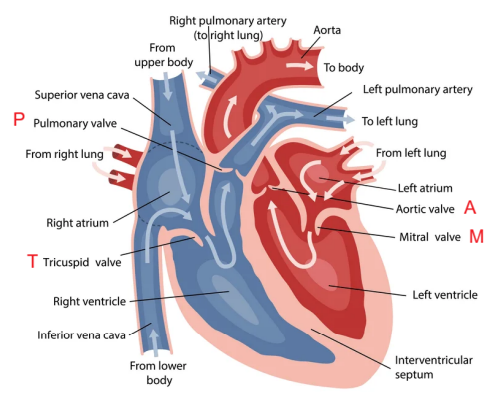
\includegraphics[width=0.8\textwidth]{docs/assignments/Final report/figures/module_2/heartimage.png}
    \caption{Cross section of a human heart \cite{IP3Man}.}
    \label{fig:heartimage}
\end{figure}

The heart can be split in a right half and a left half (from the perspective of the heart), where the T and P valves are in the right half and the M and A valves are in the left half (see Fig. \ref{fig:bloodsys}). These halves both facilitate the flow of blood using a pumping mechanism composed of the contraction of two chambers: the atrium and the ventricle. The valves are present between the atrium and the ventricle and between the ventricle and the artery, to prevent blood from flowing in the wrong direction (Fig. \ref{fig:heartschem}. While a chamber is contracting, the valve opens and allows blood to flow. When the chamber is finished contracting, the valves closes, which creates a sound wave. As the T and M valve close at around the same time, the sound they create together is called the S1 peak, as the sounds of the valve separate are hard to distinguish. The A and P valve also close at around the same time, and thus the sound they create together is called the S2 peak.

\begin{figure} [H]
    \centering
    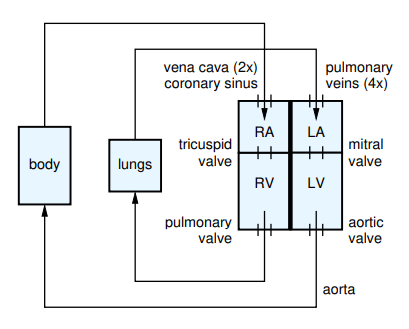
\includegraphics[width=0.8\textwidth]{docs/assignments/Final report/figures/module_2/bloodsystem.png}
    \caption{Schematic of the blood circulation system \cite{IP3Man}.}
    \label{fig:bloodsys}
\end{figure}


\begin{figure} [H]
    \centering
    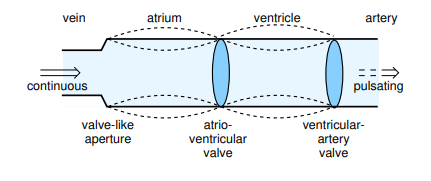
\includegraphics[width=0.8\textwidth]{docs/assignments/Final report/figures/module_2/heartschem.png}
    \caption{Schematic of atrium and ventricle \cite{IP3Man}.}
    \label{fig:heartschem}
\end{figure}


\section{Single valve model}
To model the sounds created by the heart, the sounds that each valve creates separately were modeled first. This was done by modeling an initial burst of energy (onset) and the damping out of that energy (decay). 

The damping out was modeled using a complex pole pair in the right hand side of the complex plane to create a transfer function using the following formula:
\begin{equation}
    \label{eq:transferfunction}
    H(s) = \frac{\Omega_0}{(s+a)^2+\Omega_0}
\end{equation}

This results in the following impulse response: 
\begin{equation}
    \label{eq:lhsimpulseresponse}
    h(t) = e^{-at}sin(\Omega_0 t)u(t)
\end{equation}

It can be seen that the impulse response is an oscillating decaying exponential, characterized by the parameter $a$ and $\Omega_0$, which indicate the damping and frequency, respectively. The values for these parameters will be determined later.

In order to model the initial energy of the sound, also called the onset, a complex pole pair in the right hand side of the complex plane was used. This resulted in the following impulse response:
\begin{equation}
    \label{eq:rhsimpulseresponse}
    h(t) = e^{at}sin(-\Omega_0 t)u(-t)
\end{equation}
The values of the parameters $a$ and $\Omega_0$ for the onsets will also be determined later.

\section{Multiple valves}
In order to combine the valves into one model, it must be known in what order they create the sounds and what the duration of each sound is. This was done by adjusting these parameters by comparing it to a given recording of the sounds. It was assumed that for the recording the placement of the valves didn't result in any difference in delay and damping, which is why the model could directly be compared to this recording. The $a$ and $\Omega_0$ parameters for the onset and decay of each valve were also determined using this methodology. The parameters chosen resulted in the model shown in Fig. \ref{fig:modeled_signal}.

\begin{figure} [H]
    \centering
    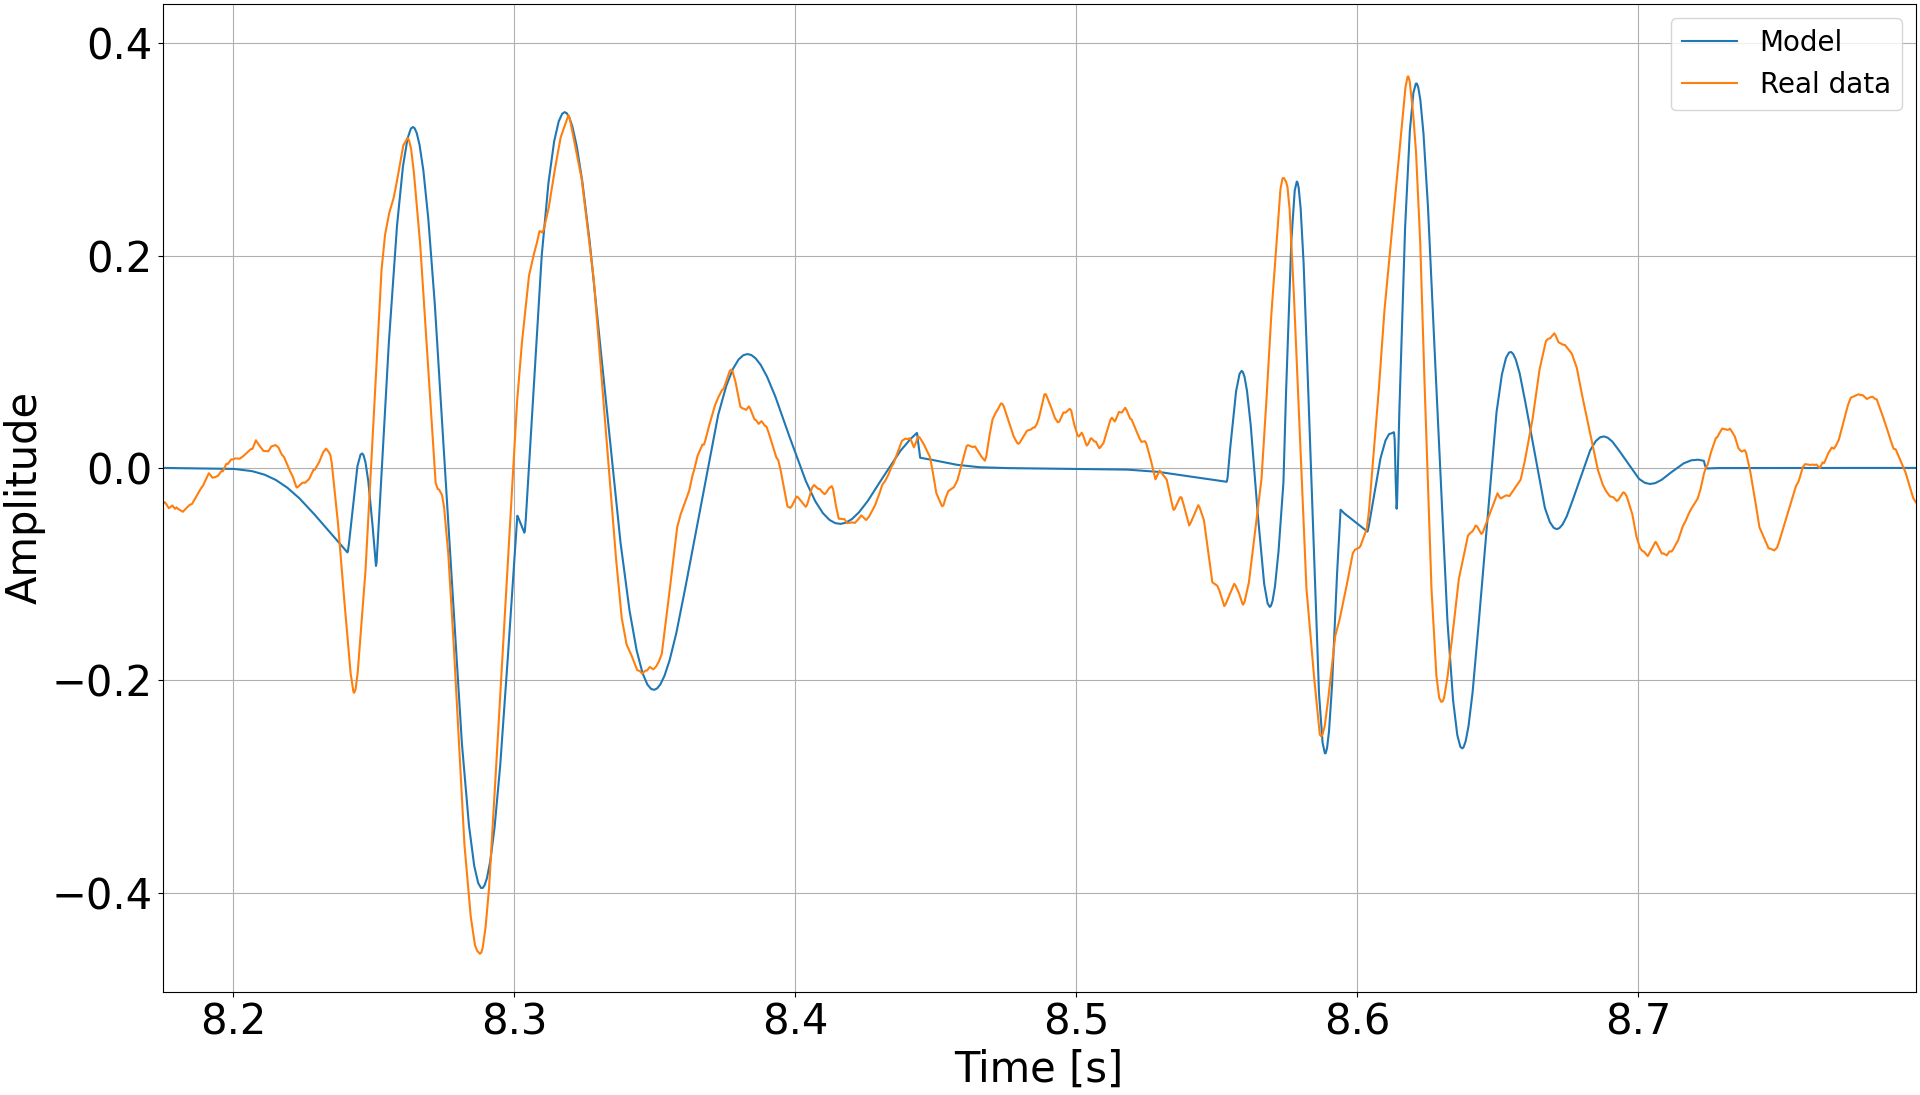
\includegraphics[width=0.9\textwidth]{docs/assignments/Final report/figures/figures/module_2/Modeled_signal.png}
    \caption{Measurement of one heart beat and the signal of the resulting single valve models combined.}  
    \label{fig:modeled_signal}
\end{figure}

In Fig. \ref{fig:suggested}, the model is plotted using the suggested parameters by \cite{IP3Man}. This is notably different from a measured heartbeat, but might be an easier signal to be processed by later systems. 

\begin{figure} [H]
    \centering
    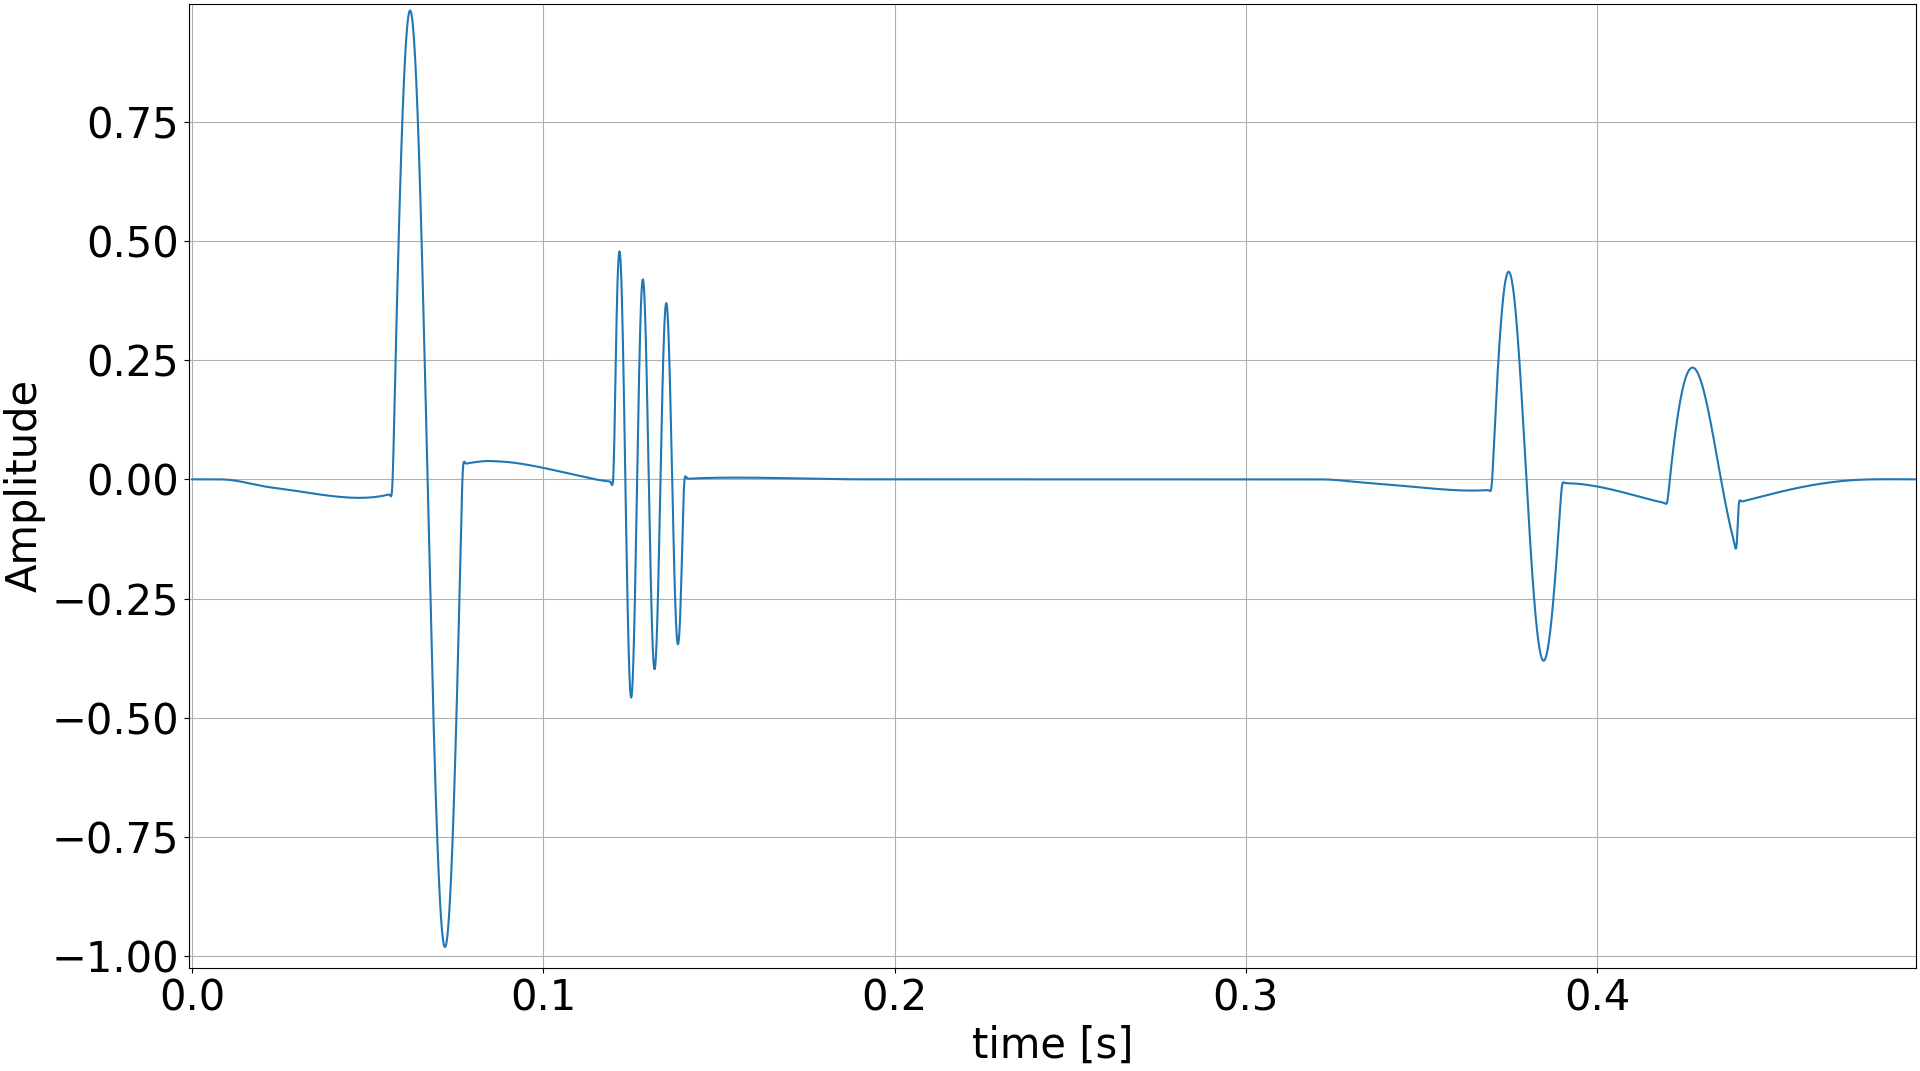
\includegraphics[width=0.85\textwidth]{docs/assignments/Final report/figures/module_2/suggested_params.png}
    \caption{The modeled signal of one heartbeat using the suggested parameters by \cite{IP3Man}.}  
    \label{fig:suggested}
\end{figure}



\section{3D model}

In order to model the damping and delay caused by the positioning of the valves, the distance between each valve and microphone pair was used. For this distance, the location of the valves were arbitrarily set to values that we seemed to be realistic. 
The damping is directly proportional to the distance, which was modeled by applying a corresponding multiplication factor. The delay is due to the speed of the signal, which was assumed to be constant throughout the medium between the microphones and the valves. 
To create modeled signals for each microphone, the signals including delay and damping of each valve were added together for each microphone, as the distance from each valve to each microphone is different.

\section{Results}
\todo{single valve time:freq plot using table values}
\todo{test segmentation on heart model.}


Fig. \ref{fig:single_valve} shows the time and frequency plot of a single valve, in this case the M valve, using parameters recommended in \cite{IP3Man}. Mostly low frequencies are present, which is to be expected as the main frequency as suggested by \cite{IP3Man} to use for the M valve is 50Hz. The shape of the time plot also seems to be correct, as it should be a decaying sinusoid, which is seen as the right peak has a lower absolute amplitude than the left peak.


\begin{figure} [H]
    \centering
    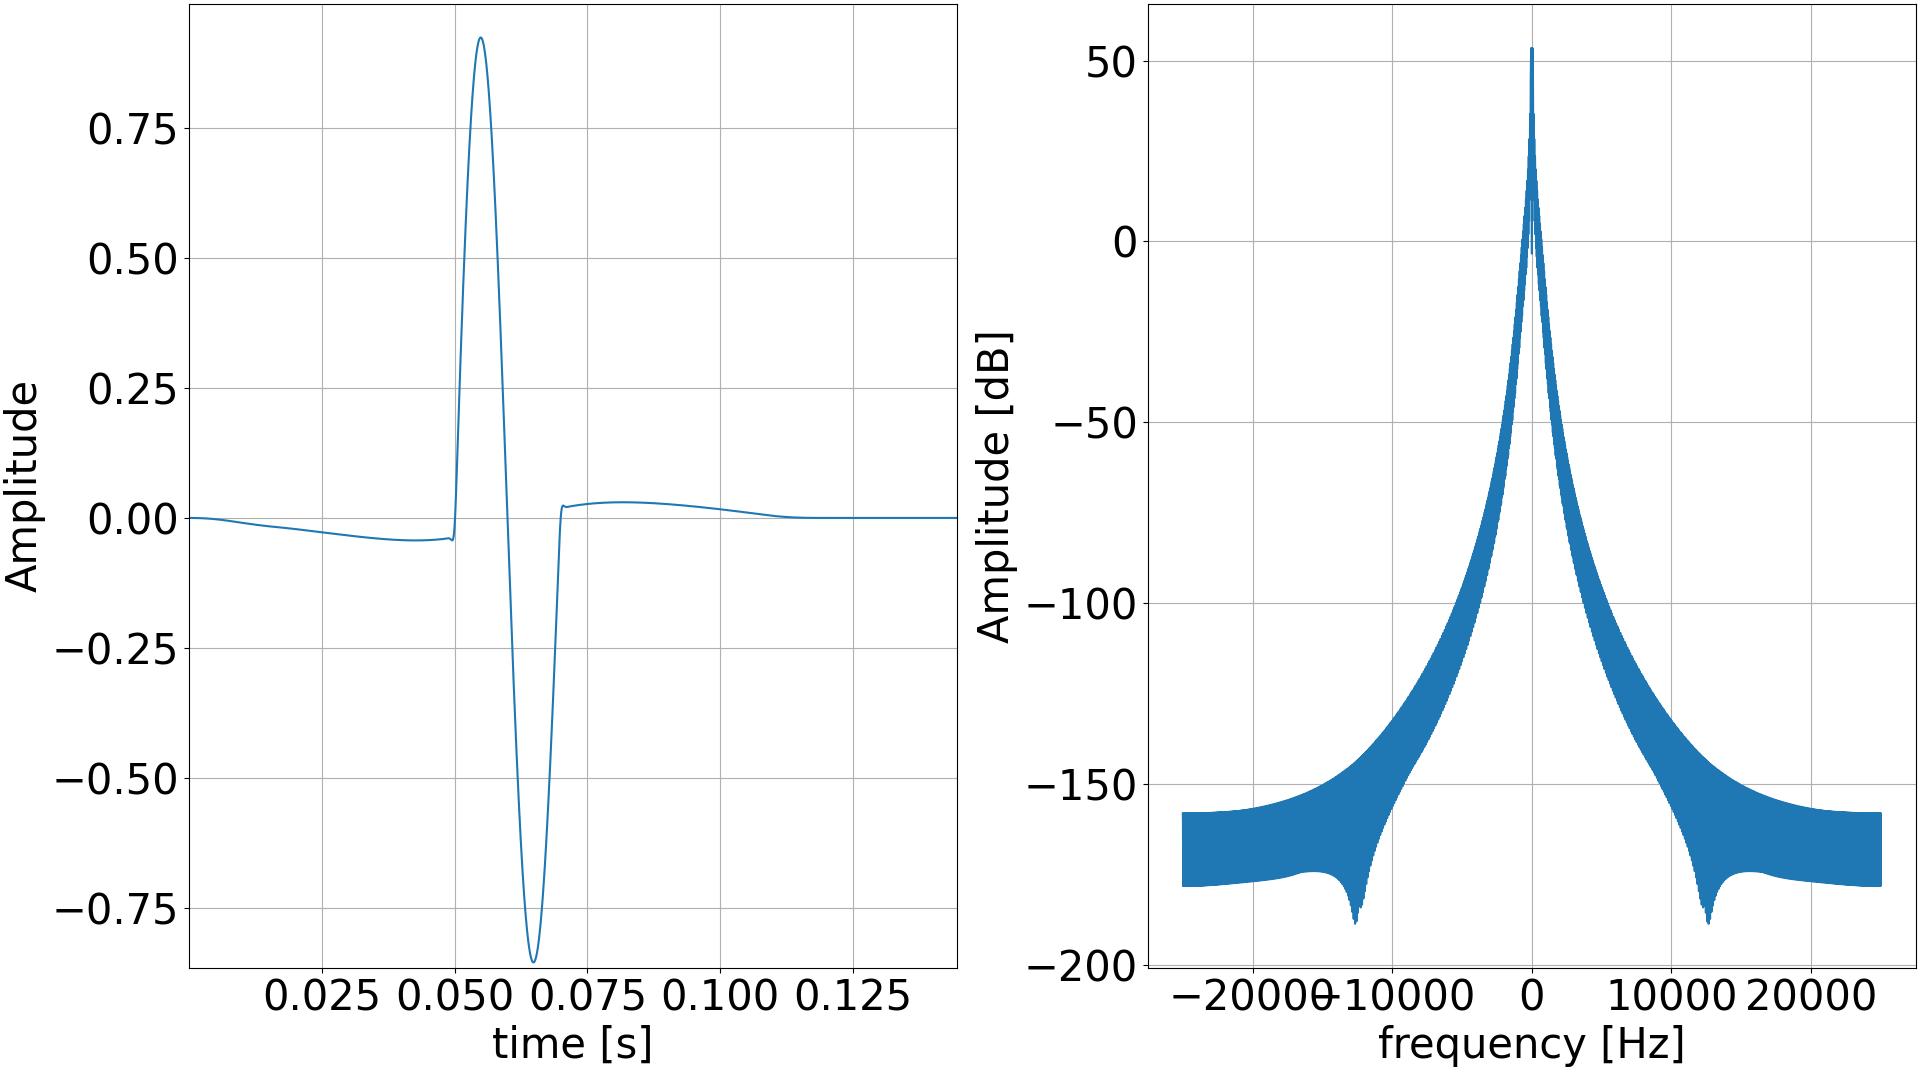
\includegraphics[width=0.85\textwidth]{docs/assignments/Final report/figures/module_2/single_valve.png}
    \caption{Time and frequency plot of a single modeled heart valve (M valve).}  
    \label{fig:single_valve}
\end{figure}



In Fig. \ref{fig:multichannel_damping} and Fig. \ref{fig:multichannel_delay} the resulting signals for the microphones have been displayed using the 3D model. The difference in damping is visible in Fig. \ref{fig:multichannel_damping} as the peaks have different heights. The difference in delay is visible in Fig. \ref{fig:multichannel_delay}, as the signals cross 0 amplitude at a different times. However, it is apparent that this delay is at most 0.5 milliseconds.

\begin{figure} [H]
    \centering
    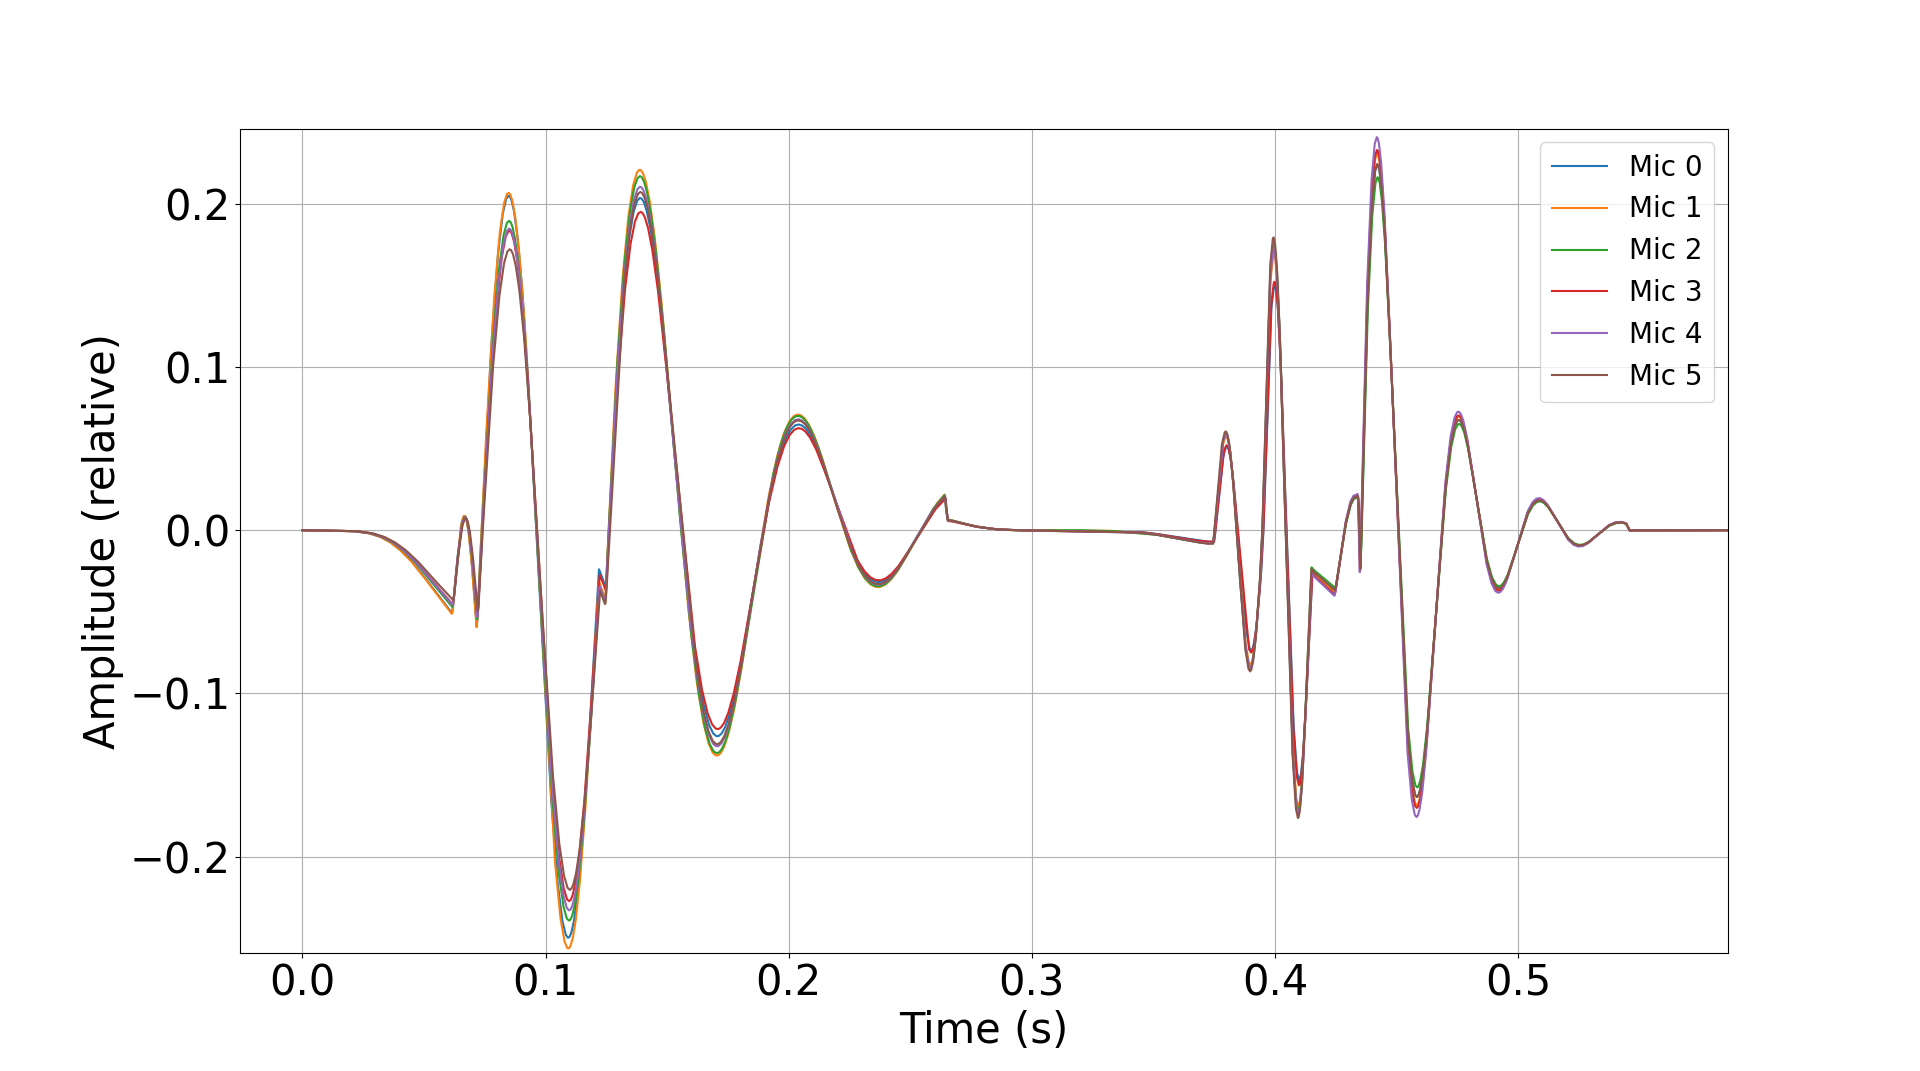
\includegraphics[width=0.95\textwidth]{docs/assignments/Final report/figures/module_2/multichannel_damping.png}
    \caption{Modeled signal for each microphone.}  
    \label{fig:multichannel_damping}
\end{figure}

\begin{figure} [H]
    \centering
    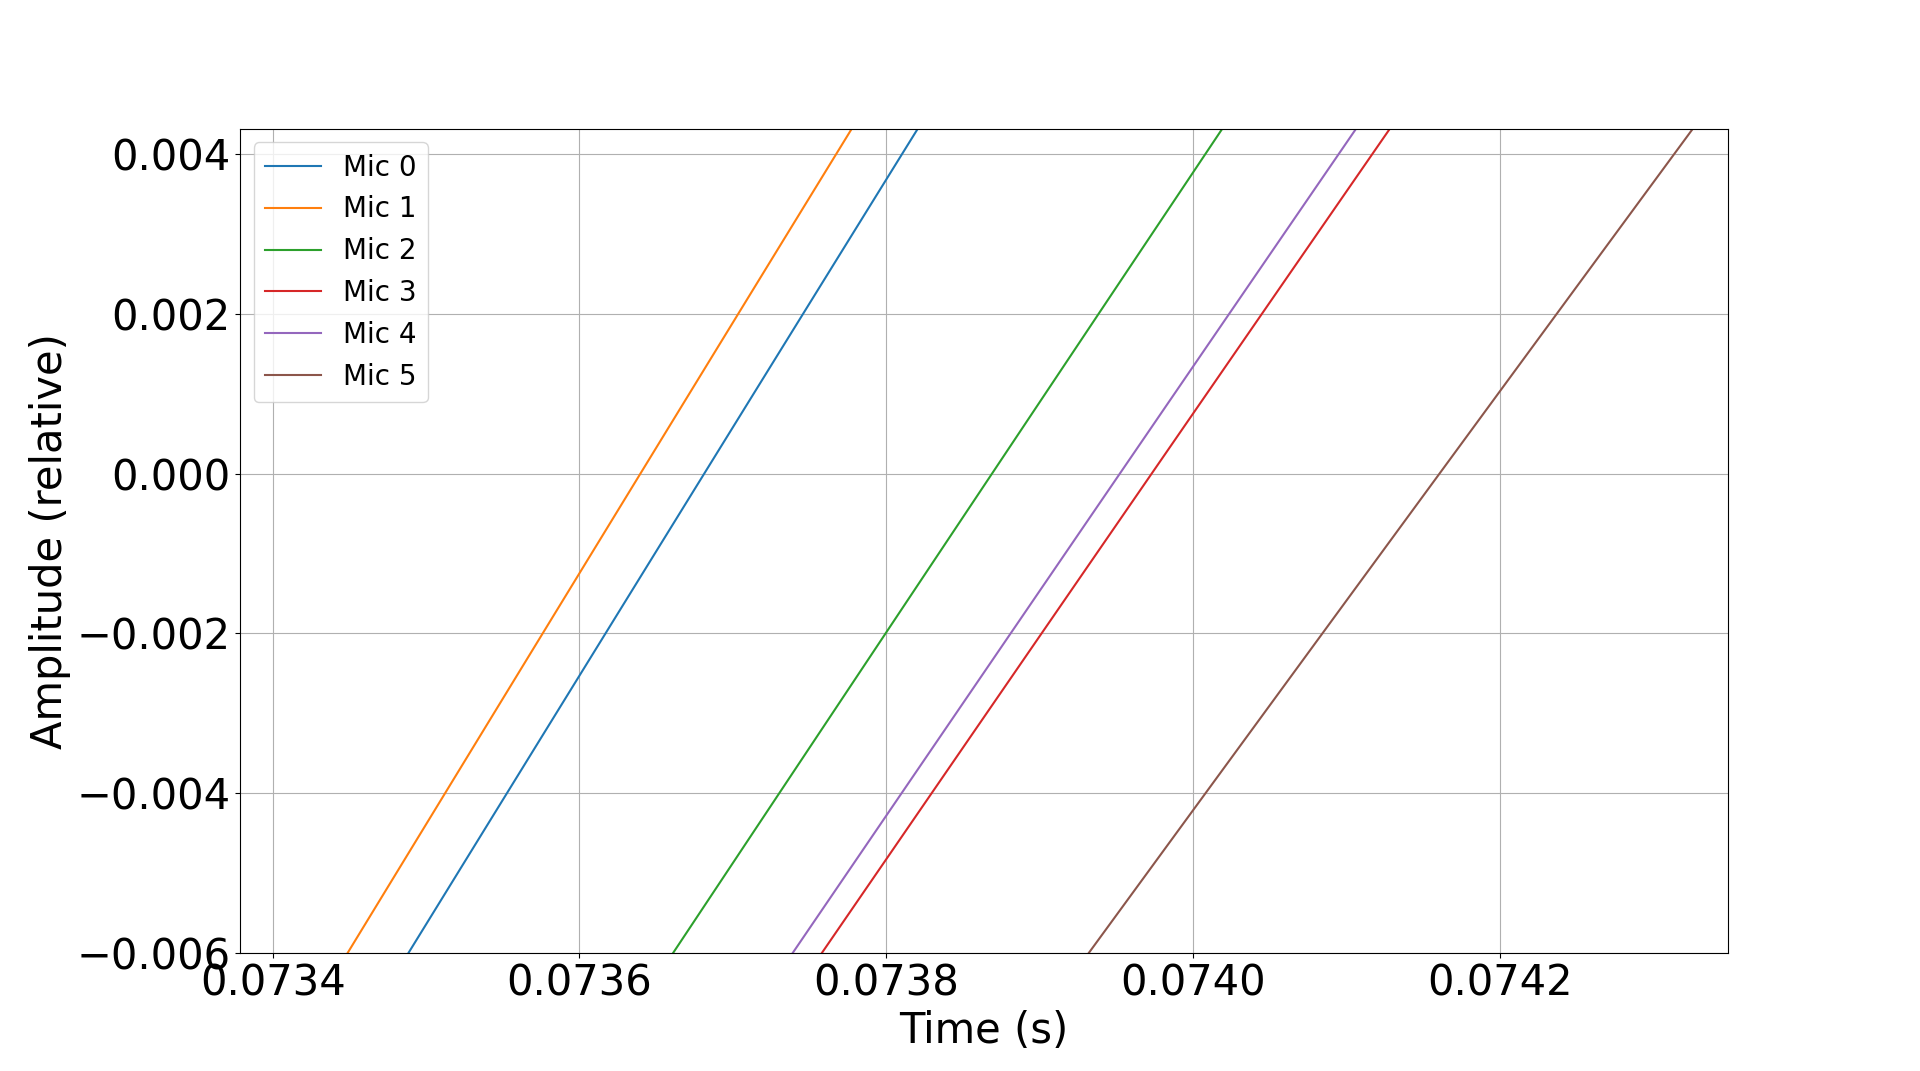
\includegraphics[width=0.95\textwidth]{docs/assignments/Final report/figures/module_2/multichannel_delay.png}
    \caption{Modeled signal for each microphone. Same data as Fig. \ref{fig:multichannel_damping}, but zoomed in.}  
    \label{fig:multichannel_delay}
\end{figure}

\section{Randomization and noise}
No two heart beats are identical, which can be modeled by randomizing the parameters that were used to generate the signals slightly. The microphone will also pick up other signals, which can be modeled by white noise. These additions resulted in the signals in Fig. \ref{fig:multichannel_random}. The noise is clearly visible, as between the heartbeats the signal oscillates about 0.02 from the baseline. The randomization becomes clear as corresponding peaks in the two heart beats are not all at the same height.

\begin{figure} [H]
    \centering
    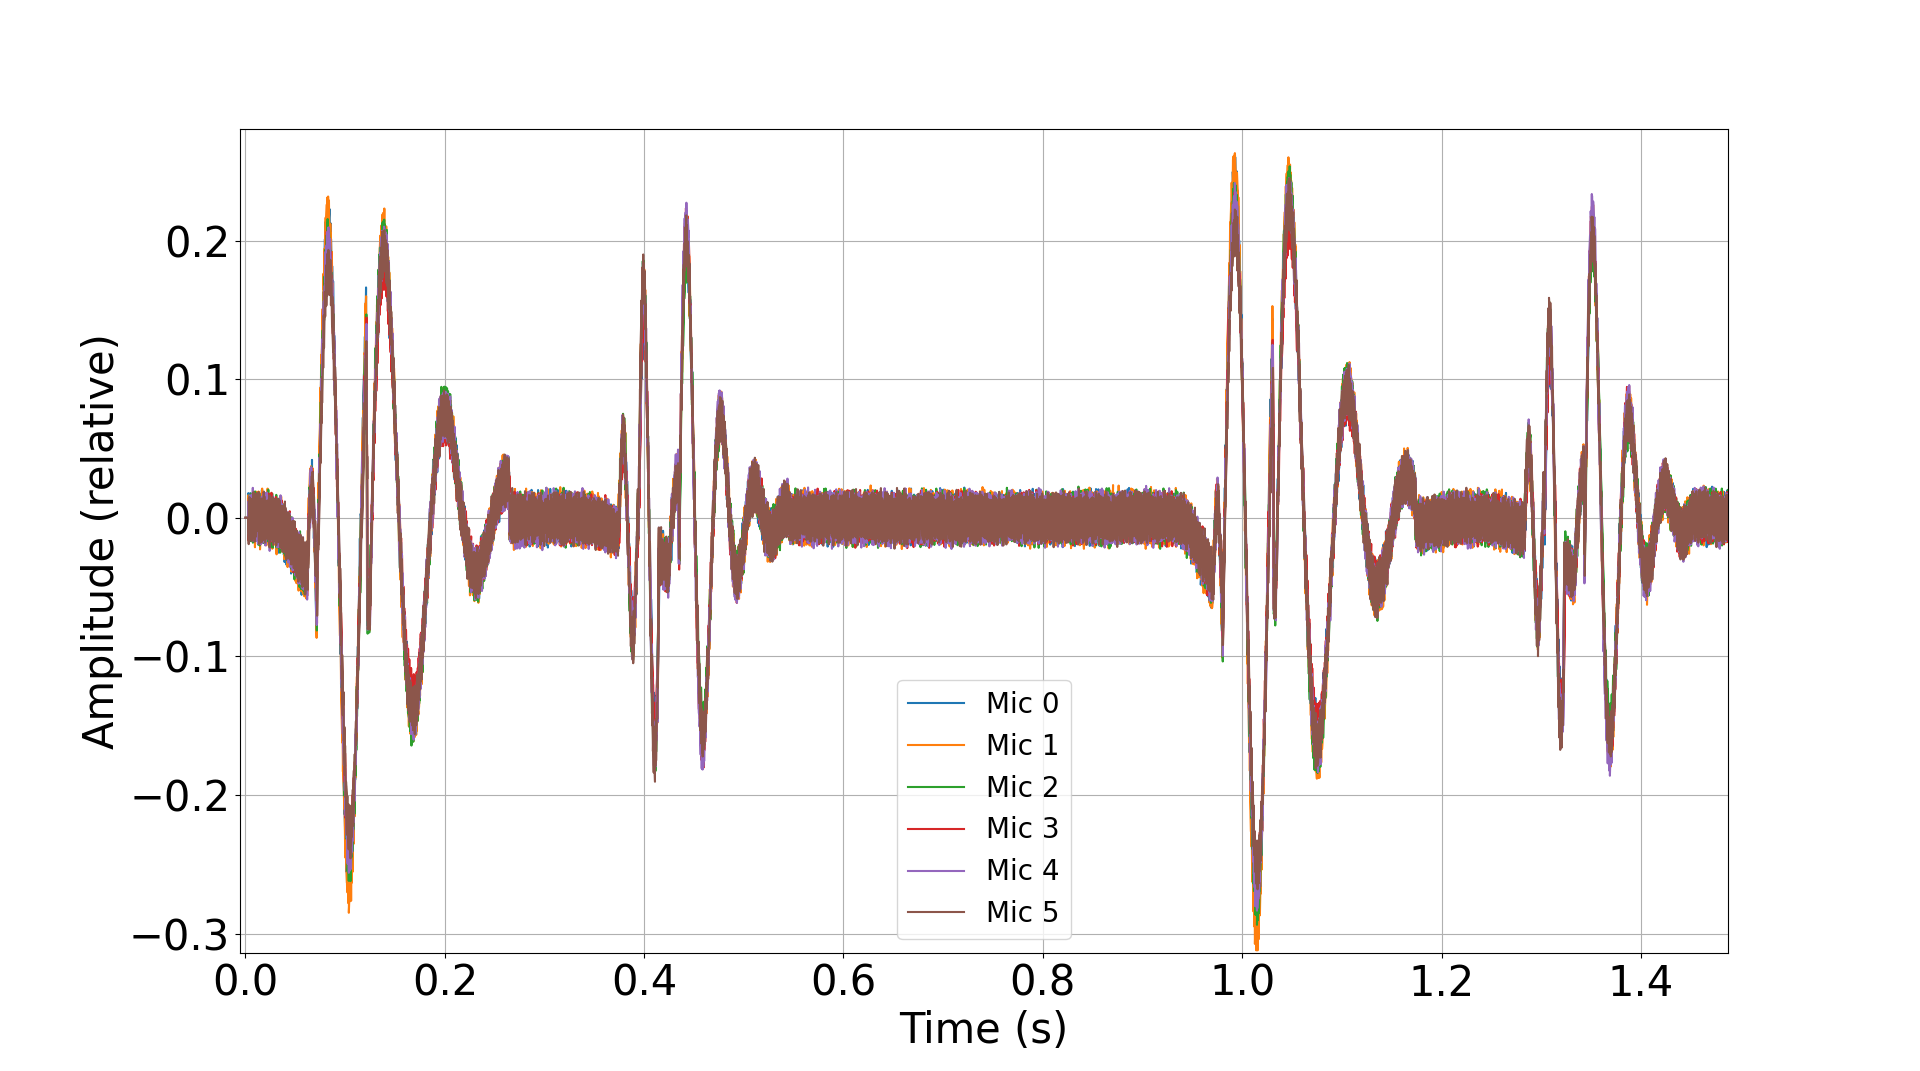
\includegraphics[width=1\textwidth]{docs/assignments/Final report/figures/module_2/multichannel_random.png}
    \caption{Modeled signal for each microphone, including randomization and noise.}  
    \label{fig:multichannel_random}
\end{figure}

\section{Conclusion}
All in all, a model of the human heart was created to simulate the sounds that it creates. This model was then applied in a 3D setting, thus creating simulated signals that the six microphones should measure. As these signals are based on known parameters, they can be used to test other algorithms.

